\section{Unified Agentic Reinforcement Learning Environment}\label{app:rl_infra}

\begin{figure}[htbp]
    \centering
    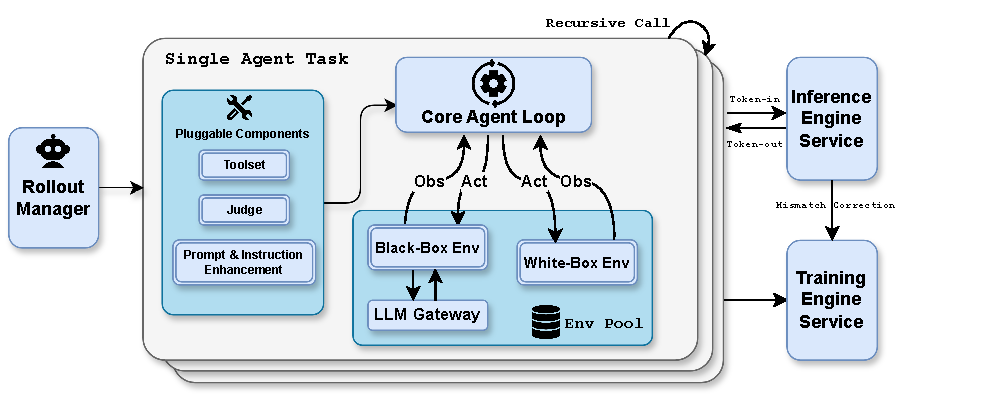
\includegraphics[width=.8\linewidth]{figures/rl_framework.pdf}
    \caption{Overview of our agentic RL framework.}
    \label{fig:rl-framework}
\end{figure}
\paragraph{Environment}
To support unified Agentic RL, our RL framework features a standardized Gym-like \cite{openaigym2016} interface to streamline the implementation of diverse environments. Such design empowers users to implement and customize environments with minimal overhead. Our design prioritizes compositional modularity by integrating a suite of pluggable components, such as a $\textit{Toolset}$ module for supporting various tools with sandboxes, a $\textit{Judge}$ module for multi-faceted reward signals, and specialized modules for prompt diversification and instruction-following enhancement. These components can be dynamically composed with core agent loops, offering high flexibility and enhancing model generalization.

At the execution level, our RL framework treats every agent task as an independent asynchronous coroutine. Each task can recursively trigger sub-task rollouts, simplifying the implementation of complex multi-agent paradigms such as \textit{Parallel-Agent RL} and \textit{Agent-as-Judge}. As shown in the figure \ref{fig:rl-framework}, a dedicated \texttt{Rollout Manager} orchestrates up to 100,000 concurrent agent tasks during the RL process, providing fine-grained control to enable features like partial rollout \cite{team2025kimi}. Upon activation, each task acquires an environment instance from a managed pool, equipped with a sandbox and specialized tools. 

\paragraph{Inference Engine Co-design}
Our framework strictly follows a \textit{Token-in-Token-out} paradigm. We also record log probabilities for all inference engine outputs to perform train-inference mismatch correction, ensuring stable RL training. A co-design of inference engine for RL requirements has allowed us to support these features by custom inference APIs for RL.

Besides a comprehensive suite of built-in white-box environments, there are also black-box environments that can only run under standard LLM API protocol, missing the opportunity to use advanced features offered by our custom API protocol. To facilitate model optimization under black-box environments, 
we developed \textit{LLM Gateway}, which is a proxy service that keeps detailed records of rollout requests and responses under our custom protocol.  

\paragraph{Monitoring and debugging} It is a challenging task to optimize performance of a highly-parallel asynchronous execution system, while ensuring correctness. We develop a series of tools for performance monitoring, profiling, data visualization and data verification. We found these to be instrumental in debugging and ensuring both the efficiency and correctness of our Agentic RL.
